\section{Samouczek}

Ostatnim z ekranów aplikacji jest samouczek, do którego bezpośredni dostęp został zapewniony z poziomu ekranu domowego.

Do jego wykonania wykorzystano wbudowany szablon \emph{TemplateScreen}, który składa się z dwóch pionowych pól - tekstowego z lewej strony oraz multimediów z prawej. Na widok całości składają się dodatkowo ikony strzałek, umożliwiających nawigację po kolekcji tekstów oraz nawigatora, prezentującego aktualny postęp prezentacji samouczka.

Obraz \ref{fig:tutorial} przedstawia przykładowy widok działania samouczka.

\begin{figure}[H]
    \centering
    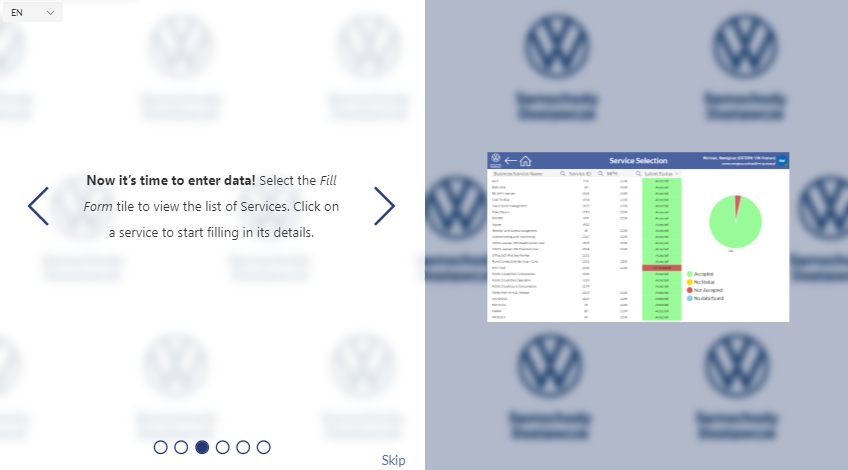
\includegraphics[width=0.75\textwidth]{figures/Tutorial.png}
    \caption{Prezentacja widoku samouczka \emph{GenerateRaport}}
    \label{fig:tutorial}
\end{figure}

\subsection{Nawigacja po samouczku}

\lstset{language=C,caption={Kod wywoływany podczas realizacji przycisku nawigacji po samouczku -- przycisk następnego elementu},label=lst:TutorialNavigate}
\begin{lstlisting}[language=PowerFx]
Set(guideStep; Min(guideStep+1; Last(TutorialNavigator1.AllItems).Step))
\end{lstlisting}

W kodzie \ref{lst:TutorialNavigate} nawigacji, funkcja \emph{Set()} jest wykorzystana do aktualizacji zmiennej \emph{guideStep}, która przechowuje wartość aktualnego kroku samouczka. Funkcja \emph{Min()} zapewnia, że wartość zmiennej kroku nie przekroczy ostatniego możliwego kroku.  Analogicznie działanie wykorzystano dla nawigacji wstecz (strzałka w lewo).

\subsection{Prezentacja zawartości w samouczku}

W samouczku opisano wszystkie ekrany w kolejności postępu procesu. Każdy z opisów znajduje się w kolekcji tekstów, jako osobny element.

\lstset{language=C,caption={Kod pobierający elementy tekstowe z kolekcji},label=lst:TutorialText}
\begin{lstlisting}[language=PowerFx]
If(IsBlank(guideStep); First(TutorialNavigator1.AllItems).Text; LookUp(TutorialNavigator1.AllItems; Step = guideStep).Text);
\end{lstlisting}

W kodzie \ref{lst:TutorialText}, funkcja \emph{If()} sprawdza, czy zmienna \emph{guideStep} jest pusta -- jeśli tak, to pobierany jest pierwszy element z kolekcji \emph{TutorialNavigator1.AllItems} za pomocą \emph{First()}. W przeciwnym razie, funkcja \emph{LookUp()} wyszukuje element o pasującym numerze kroku, zwracając odpowiadający tekst.

\subsection{Prezentacja grafik w samouczku}

Analogicznie jak w przypadku wyświetlania tekstu, grafiki ilustracyjne aplikacji są dynamicznie pobierane zgodnie z postępem nawigacji. Każdy z etapów samouczka zawiera odpowiedni obrazek, który wyświetlany jest razem z przypisanym do niego tekstem.